\documentclass[a4paper,12pt]{scrartcl}

\usepackage[T1]{fontenc}
\usepackage{lmodern}
\usepackage[utf8]{inputenc}
\usepackage[french]{babel}
\usepackage{graphicx}
\usepackage{microtype} 
\usepackage[onehalfspacing]{setspace}
\usepackage[top=2.5cm, bottom=2.5cm, left=3cm, right=3.5cm]{geometry}
\usepackage{tabularx}
\usepackage{graphicx}
\usepackage{longtable}
\usepackage{listings}
\usepackage{listingsutf8}
\usepackage{dsfont}
\usepackage{appendix}
\usepackage{amsmath}
\usepackage{hyperref}
\usepackage{mathtools, amssymb}
\usepackage[usenames,dvipsnames]{color}

% \begin{equation}
% \begin{split}
%     \dbx & =\dbx[3cm] \\
%     & =\dbx
% \end{split}
% \end{equation}

\definecolor{MyDarkGreen}{rgb}{0.0,0.4,0.0}
\lstloadlanguages{Matlab}
\lstset{language=Matlab,                        % Use MATLAB
        frame=single,                           % Single frame around code
        basicstyle=\small\ttfamily,             % Use small true type font
        keywordstyle=[1]\color{Blue}\bfseries,  % MATLAB functions bold and blue
        keywordstyle=[2]\color{Purple},         % MATLAB function arguments purple
        keywordstyle=[3]\color{Blue}\underbar,  % User functions underlined and blue
        identifierstyle=,                       % Nothing special about identifiers
                                                % Comments small dark green courier
        commentstyle=\usefont{T1}{pcr}{m}{sl}\color{MyDarkGreen}\small,
        stringstyle=\color{Purple},             % Strings are purple
        showstringspaces=false,                 % Don't put marks in string spaces
        tabsize=5,                              % 5 spaces per tab
        %
        %%% Put standard MATLAB functions not included in the default
        %%% language here
        morekeywords={xlim,ylim,var,alpha,factorial,poissrnd,normpdf,normcdf},
        %
        %%% Put MATLAB function parameters here
        morekeywords=[2]{on, off, interp},
        %
        %%% Put user defined functions here
        morekeywords=[3]{brownmo},
        %
        morecomment=[l][\color{Blue}]{...},     % Line continuation (...) like blue comment
        numbers=left,                           % Line numbers on left
        firstnumber=1,                          % Line numbers start with line 1
        numberstyle=\tiny\color{Blue},          % Line numbers are blue
        stepnumber=5,                           % Line numbers go in steps of 5
        literate=%                              % accents and Umlaute
                 {Ö}{{\"O}}1
                 {Ä}{{\"A}}1
                 {Ü}{{\"U}}1
                 {ß}{{\ss}}1
                 {ü}{{\"u}}1
                 {ä}{{\"a}}1
                 {ö}{{\"o}}1
                 {\$}{{\dollar}}1
        }

\title{Mini projet 1: Calcul du prix d'une option asiatique}
\author{Valentin DE CRESPIN DE BILLY \\ Matthias LANG}
\date{30.11.2021}

\linespread{1.5} 


\begin{document}

\maketitle
\begin{center}

  \thispagestyle{empty}

  N. d'étudiant: 247067 et 313411\\
  Université Catholique de l'Ouest\\
  Mathématiques financières

\end{center}

\newpage

\section{Calculer le prix du sous-jacent}

Nous avons essayé d'atteindre une équation qui ne dèpend que des variables connues comme la formule de Black-Scholes.
Cela n'a pas fonctionné.

\begin{align}%equation} \label{1} 
dS_t  &=  S_t(rdt+\sigma \sqrt{S_t} dW_t) \\
     \iff \frac{dS_t}{S_t}  &=  rdt+\sigma \sqrt{S_t} dW_t
\end{align}


On prend l'équation 1:
%\begin{equation} \label{3}
%\begin{multlined}
\begin{align*}
= dS_t~=~S_trdt+\sigma S_t^{1.5} dW_t ~~
\text{; Puis} \\
d \langle S_t &, ~ S_t\rangle \\
=\langle dS_t &,~ dS_t\rangle ~=\\
=\langle S_trdt+\sigma S_t^{1.5} dW_t &,~
         S_trdt+\sigma S_t^{1.5} dW_t \rangle ~=\\
=\langle \sigma S_t^{1.5} dW_t &,~
         \sigma S_t^{1.5} dW_t \rangle ~=\\
=S_t^3 \sigma^2 \langle dW_t &,~  dW_t \rangle ~=\\
=S_t^3 \sigma^2 dt
\end{align*}


On pose: 
$X_t = ln(S_t)$
%\begin{equation} \label{4}
%\begin{multlined}
\begin{align}
\text{Formule d'Ito: } dln(S_t) = \frac{dS_t}{S_t} + \frac{1}{2} \frac{-1}{S_t^2}d \langle S_t, ~S_t \rangle \\
\end{align}
Avec les équations 2 et 3:
\begin{align}
dln(S_t) = 
rdt + \sigma \sqrt{S_t} dW_t - \frac{1}{2}S_t \sigma^2 dt =
(r - \frac{1}{2}S_t\sigma^2)dt + \sigma\sqrt{S_t}dW_t
\end{align}


\begin{align*}
ln( \frac{S_t}{S_0} ) 
&= ln(S_t)-ln(S_0) = \int_0^t dln(S_u) = \\
&= \int_0^t (r-\frac{1}{2} S_t \sigma^2)du~+~\int_0^t \sigma \sqrt{S_t}dW_t \\
&=\dots
\end{align*}
Donc on ne peut pas facilement dériver une formule pour le prix comme ça, qui dépend que des variables fixées, mais on peut le simuler pas à pas en utilisant (1):

\begin{equation} \label{6}
\begin{split}
S_0  &~\text{soit connu} \\
dS_0 &= S_0(rdt + \sigma \sqrt{S_0} dW_0) \\
S_1  &\approx S_0 + dS_0 \\
dS_1 &= S_1(rdt + \sigma \sqrt{S_1} dW_1) \\
S_2  &\approx S_1 + dS_1 \\
\dots
\end{split}
\end{equation}


\subsection{ecdf}
Sieht Gaussian aus -> KI damit probieren, aber keine richtige Normalverteilung, also bootstrap!

\subsection{Réduction de la variance du éstimateur}

Les éstimateurs ont une variance telle que:
$ \hat{Var}(C) = \hat{\sigma_i^2} / n_t$, oú $n_t$ est le nombre des observations et $\hat{\sigma_i^2}$ est la variance estimée de la population, qui est égal à la variance de l'échantillon.

Supposons que nous ne connaissions ni les paramètres ni la règle à partir desquels les prix sont établis. 
Nous ne pouvons donc pas augmenter le nombre d'observations pour améliorer l'estimateur.
Quelle autre possibilité existe-t-il pour réduire sa variance ?

Avec les techniques de bootstrap on pourrait répliquer les données. 
Mais on risque de introduir un biais.
Si on utilise une variable de contrôle on n'invente pas des nouvelles données, ni risque-t-on de changer l'ésperance.

% variable antith

\section{Réalisation numerique}

Les algorithmes sont réalisées avec deux langues de programmation: Matlab et Visual Basic for Applications.
Plusieurs graphiques sont y générés, vous les trouverez dans l'annexe \ref{graphiques}.
En plus, avec le logiciel Excel nous avons crée un dashboard, voir une capture d'figure ref{X}. 
Vous trouverez les scriptes et les images dans l'annexe, et avec la fiche de dashboard également dans le \href{https://github.com/matthias-10/UCO_actuariat_mini-projet}{repository}.


\subsection{Variable antithétique}
\subsection{Variables de contrôle}

Afin de réaliser une réduction de variance de l'éstimateur, sans être contraint des ressources de calculation, on peut se servire des variables des contrôle.
Soit $X$ la variable aléatoire dont on veut obtenir l'éstimateur Monte Carlo.
Pour chaque $X_i$ on peut simuler une autre variable $Y_i$, la variable de contrôle.

Cette variable est indépendante, mais correlée avec $X$.
D'ailleurs on sait son ésperance.
Avec les deux valeurs on creer une autre série de données ainsi:
$Z_i = X_i - \lambda(Y_i - E(Y_i))$ avec $\lambda = sigma_X/sigma_Y * \rho$.

\subsubsection{Variable de contrôle 1}

La première variable est construite avec des bruits blancs, plus ou moins la même manière que le prix d'action.
Problematique: Les X et Y ne sont pas independant en utilisant le meme processus?
Non overlapping increments Wt-Ws and Wv-Wu for any 0=s<t=>u<v are independent of each other.
On ajoute $S_0$ pour que les deux puissent être comparées.
$$X_i = S_0 + sum_{i=1}^{n} W_{t_i}$$

C'est facile de démontrer l'ésperance:
$$\mathbb{E}[X_i]=\mathbb{E}[S_0 + sum_{i=1}^{n} W_{t_i}] = S_0$$

La variance, sachant que $\mathbb{E}[W_1*W_2] =\mathbb{E}[W_t_1]*\mathbb{E}[W_t_2] =0$ et $Var(W_t_1) = t_1$, donc  $cov(W_t_1, W_t_2) = t_1$:
$$var(X_i) = 
var(S_0 + sum_{i=1}^{n} W_{t_i}) = 
var(sum_{i=1}^{n} W_{t_i}) = 
\mathbb{E}[(sum_{i=1}^{n} W_{t_i})^2] = 
var(sum_{i=1}^{n} W_{t_i}) =
\sum_{i=1}^n cov(W_t_i, W_t_i) = 
\sum_{i=1}^n \sum_{j=1}^n cov(W_t_i, W_t_i) =
\sum_{i=1}^n \sum_{j=1}^i cov(W_t_i, W_t_j) + sum_{i=1}^{n-1} \sum_{j=i+1}^n cov(W_t_i, W_t_j) =
\sum_{i=1}^n \sum_{j=1}^i t_k + sum_{i=1}^{n-1} \sum_{j=i+1}^n t_i =
T(\sum_{i=1}^n \sum_{j=1}^i \frac{k}{n} + sum_{i=1}^{n-1} \sum_{j=i+1}^n \frac{i}{n}) =
\frac{T}{n}(\sum_{i=1}^n \frac{i(i+1)}{2} + sum_{i=1}^{n-1} i(n-i)) =
\frac{T}{n}(\frac{1}{6}n(n+1)(n+2)+\frac{1}{6}n(n-1)(n+1)) =
\frac{T}{6}(2n^2+3n+1)
$$

Avec cela et on calcule $\lambda$. lambda peut-être calculé avec des données différentes.
De toute façon le temps de calcul de $\lambda$ n'est pris compte dans le temps de calcul affiché.

\subsubsection{Variable de contrôle 2}
C'est pratique de remplacer la variance par sa contrepartie empirique. 
Avec un échantillon de $n=100$ on calcule ainsi le $\lambda$ avant qu'on simule les $Z_i$.
D'où on n'utilize pas trop des calculations, le temps de calcul ne sera pas biais,
et, le plus important, $Z_i$ et $\lambda$ seront indépendant des autres.

% si K proche de S_T l'estimateur est trop bas. Pourquoi ?

\subsubsection{Variable de contrôle 3}
En surplus, ces variables ne sont réalisées que en matlab.


%%%%%%%% A N N E X E %%%%%%%%%%%%%%%%%%
\clearpage

\appendix
\appendixpage
\addappheadtotoc

\begin{center}
Toutes les fiches se trouvent dans le repository en ligne: 

 \url{https://github.com/matthias-10/UCO_actuariat_mini-projet}
\end{center}

\section{Graphiques} \label{graphiques}

\begin{figure}[h!]
  \begin{center}
    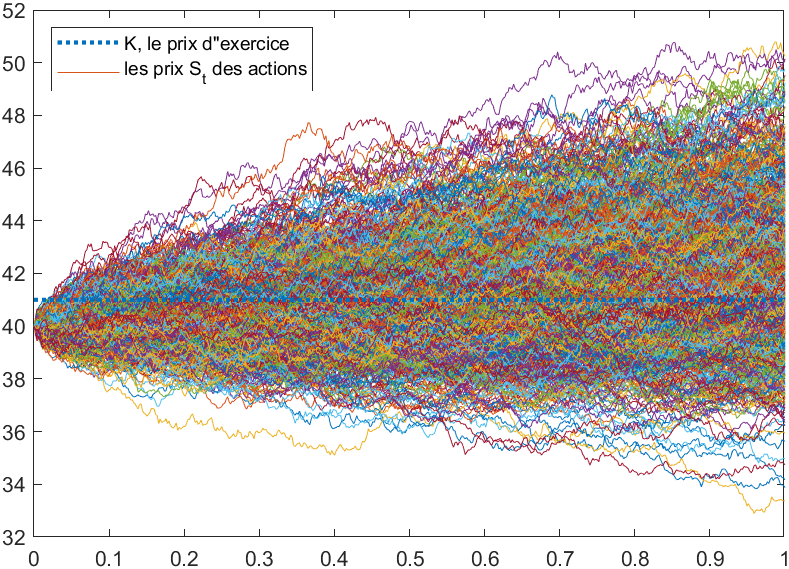
\includegraphics[width=14cm]{"graphiques/S.png"}
    \caption{Les graphes de tous trajectoires, plotés avec matlab}
    \label{fig:S}
  \end{center}
\end{figure}

\begin{figure}[h!]
  \begin{center}
    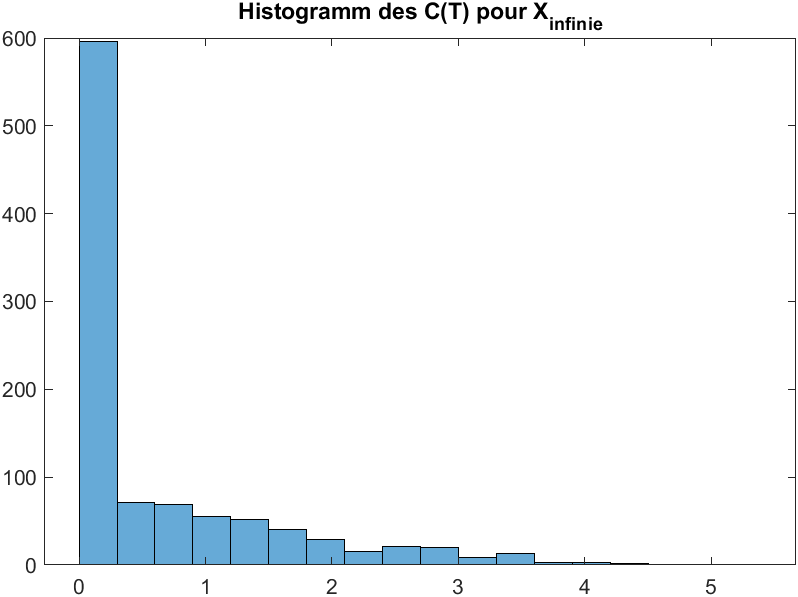
\includegraphics[width=14cm]{"graphiques/hist_C_inf.png"}
    \caption{Histogramme des simulations pour $C_{\infty}$}
    \label{fig:hist_C_inf}
  \end{center}
\end{figure}

\begin{figure}[h!]
  \begin{center}
    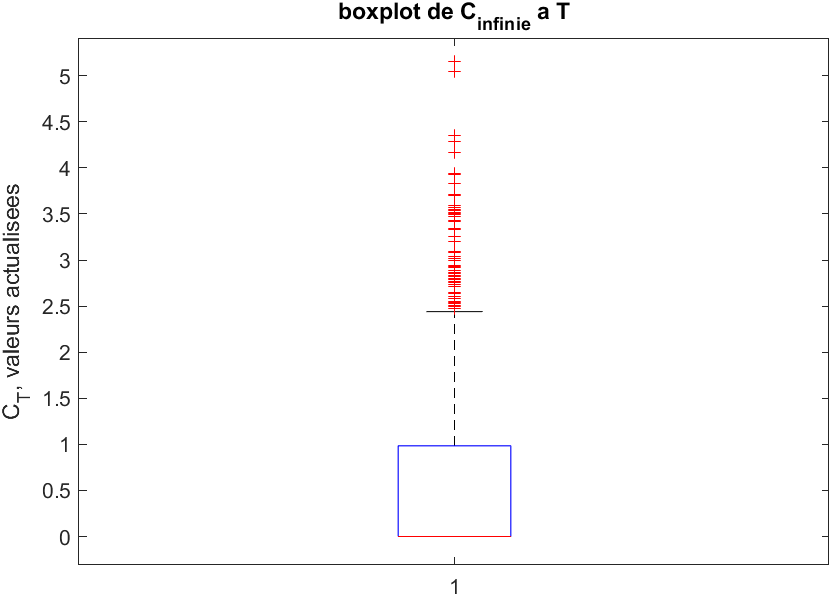
\includegraphics[width=14cm]{"graphiques/box_C_inf.png"}
    \caption{Boxplot des simulations pour $C_{\infty}$}
    \label{fig:box_C_inf}
  \end{center}
\end{figure}

\begin{figure}[h!]
  \begin{center}
    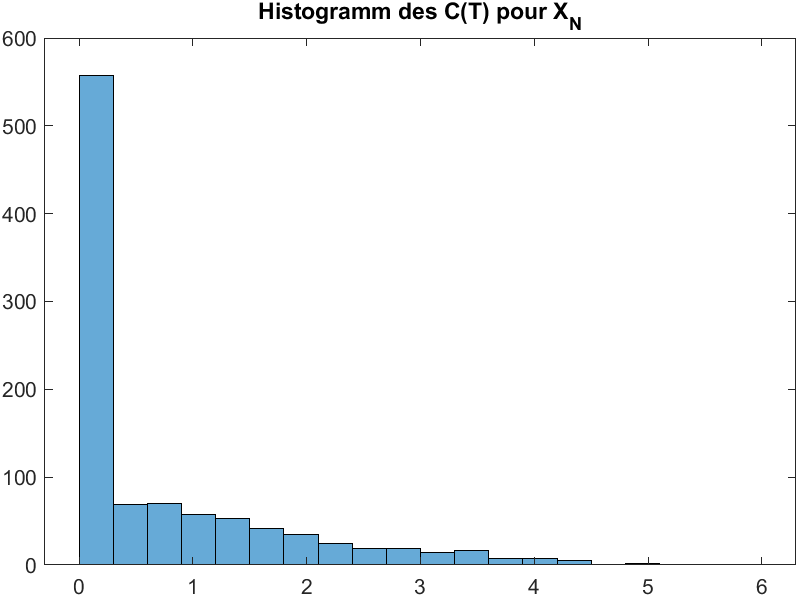
\includegraphics[width=14cm]{"graphiques/hist_C_N.png"}
    \caption{Histogramme des simulations pour $C_{N}$}
    \label{fig:hist_C_N}
  \end{center}
\end{figure}

\begin{figure}[h!]
  \begin{center}
    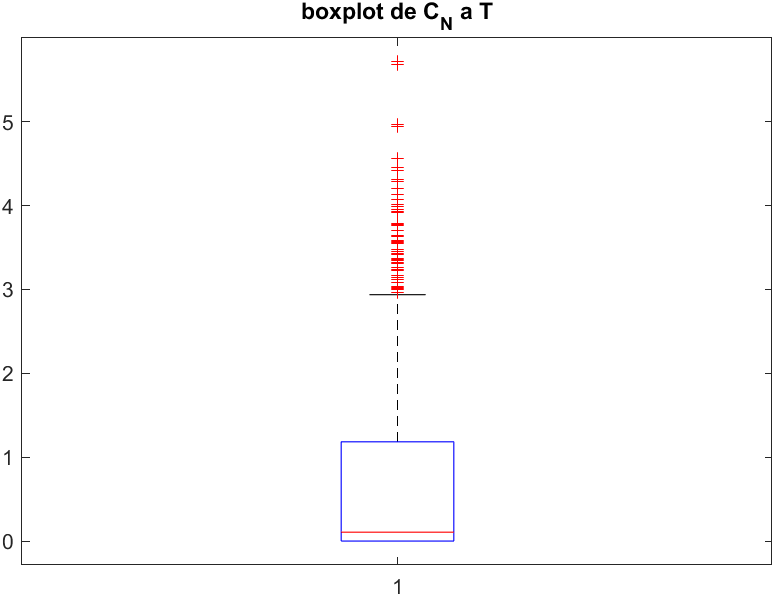
\includegraphics[width=14cm]{"graphiques/box_C_N.png"}
    \caption{Boxplot des simulations pour $C_{N}$}
    \label{fig:box_C_N}
  \end{center}
\end{figure}

\begin{figure}[h!]
  \begin{center}
    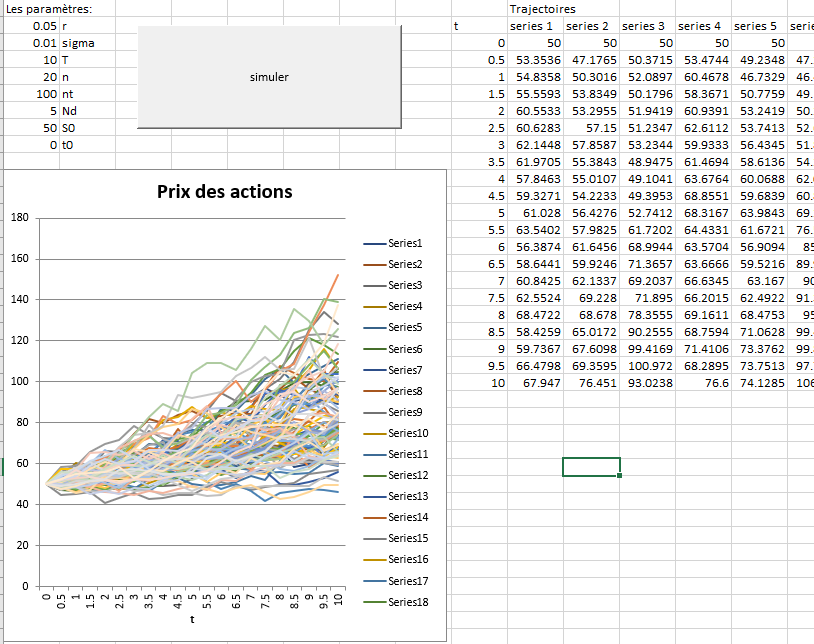
\includegraphics[width=14cm]{"graphiques/Capture.PNG"}
    \caption{le Excel dashboard}
    \label{fig:capture}
  \end{center}
\end{figure}


\section{Code Matlab}
\lstinputlisting{mini_projet.m}

\section{Code VBA}
\begin{lstlisting}[
    breaklines=true,
    tabsize=3,
    showstringspaces=false
    extendedchars=\true,
    language={[Visual]Basic},
    frame=single,
    framesep=3pt,%expand outward.
    framerule=0.4pt,%expand outward.
    xleftmargin=3.4pt,%make the frame fits in the text area. 
    xrightmargin=3.4pt,%make the frame fits in the text area.
    ]
Option Explicit

Public n, nt, Nd As Integer
Public S0, k, r, sigma, T As Double

Sub Macro1()


' worksheets
Dim sh_dash, sh_traj, sh_ic As String
Dim sh_dash_o As Worksheet
sh_dash = "Dashboard"
sh_traj = "trajectoires"
sh_ic = "IC"
Set sh_dash_o = Worksheets(sh_dash)


' ~~~~~~~~~~ parametres ~~~~~~~~~~



S0 = Range("S0_").Value
k = Range("K_").Value

r = Range("r_").Value
sigma = Range("sigma_").Value

n = Range("n_").Value
T = Range("T_").Value
Nd = Range("Nd_").Value

nt = Range("nt_").Value


Dim dt As Double
dt = T / n


Dim tps_debut, tps_passe As Double
Dim n_aff As Integer
n_aff = 10 'nombre des trajectoires affichées dans le graphique

' premier cellule de la table de trajectoires ~ t0
Dim Srow, Scol As Integer
Dim Scol_abc As String
Srow = 3
Scol_abc = "I"
Scol = 9

' iteratives
Dim i, j, l As Integer

' array pour enregistrer les simulations
Dim X() As Double 'for some reason double arrays must be defined one by one, else they are variant
Dim X_N() As Double
Dim C() As Double

Dim dW As Double
Dim a, b, e, f As Double

'effacer t et S() anciens
With Worksheets(sh_traj)
    Range(.Cells(3, 1), _
          .Cells(Srow + 10000, Scol + 10000)).Delete
End With


' afficher t
Dim temps() As Double
ReDim temps(n)
temps(0) = 0
For j = 1 To n
    temps(j) = temps(j - 1) + dt
Next

'MsgBox temps(0)
'MsgBox temps(1)
'MsgBox temps(n)
'MsgBox Application.CountA(temps)
'MsgBox UBound(temps)

Sheets(sh_traj).Range("A3:A" & UBound(temps) + 3) = _
    WorksheetFunction.Transpose(temps)


'~~~~~~~~~~~~~~~~~~ series illustratives pour l'affichage ~~~~~~~~~~~~
'~~~~~~~~~~~~~~~~~~
' pour le graphique
'~~~~~~~~~~~~~~~~~~

For j = 1 To n_aff
    i = 1
    a = S0
    
    
    'If j <= n_aff Then
        Sheets(sh_traj).Cells(Srow - 1 + i, Scol - 1 + j).Value = a
    'End If
    
    For i = 2 To n + 1
        'simuler une v.a. normale
        dW = Sqr(-2 * Log(Rnd())) * _
             Cos(6.283185307 * Rnd()) * Sqr(dt)
        a = a * (1 + (r * dt + sigma * Sqr(a) * dW))
     
        'If j <= n_aff Then
            Sheets(sh_traj).Cells(Srow - 1 + i, Scol - 1 + j).Value = a
        'End If
              
    Next
Next

'~~~~~~~~~~~~~~~~~~~~~~~~~
' pour l'exemple de series
'~~~~~~~~~~~~~~~~~~~~~~~~~

a = S0
b = S0
e = S0
f = S0


i = 1
Sheets(sh_traj).Cells(Srow - 1 + i, 2).Value = a
Sheets(sh_traj).Cells(Srow - 1 + i, 3).Value = b
Sheets(sh_traj).Cells(Srow - 1 + i, 4).Value = e
Sheets(sh_traj).Cells(Srow - 1 + i, 5).Value = f

For i = 2 To n + 1
    'simuler une v.a. normale
    dW = Sqr(-2 * Log(Rnd())) * _
         Cos(6.283185307 * Rnd()) * Sqr(dt)
    
    'le prix de l'action
    a = a * (1 + (r * dt + sigma * Sqr(a) * dW))
    
    'la variable antithetique
    b = b * (1 + (r * dt - sigma * Sqr(b) * dW))
    
    'VC_1
    e = e + dW
    
    'VC_2
    f = f + dW ' * Exp(r * (i - 1) * dt)
        
    Sheets(sh_traj).Cells(Srow - 1 + i, 2).Value = a
    Sheets(sh_traj).Cells(Srow - 1 + i, 3).Value = b
    Sheets(sh_traj).Cells(Srow - 1 + i, 4).Value = e
    Sheets(sh_traj).Cells(Srow - 1 + i, 5).Value = f
    
Next
    

'~~~~~~~~~~~~~~~~ X_inf ~~~~~~~~~~~~~~~~

tps_debut = Timer

ReDim X(1 To nt)

'simuler S pas a pas, afficher n_aff S dans sh_traj

For j = 1 To nt
    i = 1
    a = S0
    X(j) = 0.5 * a / n
    
    
    For i = 2 To n + 1
        'simuler une v.a. normale
        dW = Sqr(-2 * Log(Rnd())) * _
             Cos(6.283185307 * Rnd()) * Sqr(dt)
        a = a * (1 + (r * dt + sigma * Sqr(a) * dW))
        X(j) = X(j) + a / n
              
    Next
   
    X(j) = X(j) - 0.5 * a / n
  
Next

'Calculer C a temps 0 avec X et K
C = payoff(X)

' ~~~~~~~~~~~~~~~~~
' estimateurs X_inf
'~~~~~~~~~~~~~~~~~~

Dim C_mu, C_std, C_mu_b, C_mu_h As Double

C_mu = Mean(C)
C_std = StdDev(C)

C_mu_b = C_mu - 1.96 * C_std / Sqr(nt)
C_mu_h = C_mu + 1.96 * C_std / Sqr(nt)

tps_passe = Round(Timer - tps_debut, 3)

'affichage
Sheets(sh_ic).Range("A3").Value = "C_inf"
Sheets(sh_ic).Range("B3").Value = C_mu_b
Sheets(sh_ic).Range("C3").Value = C_mu
Sheets(sh_ic).Range("D3").Value = C_mu_h
Sheets(sh_ic).Range("E3").Value = tps_passe


'~~~~~~~~~~~~~~~~ X_N ~~~~~~~~~~~~~~~~

tps_debut = Timer

' pour X_N
ReDim X_N(1 To nt)

'simuler S pas a pas, afficher n_aff S dans sh_traj

For j = 1 To nt
    l = 1
    i = 1
    a = S0
    X_N(j) = 0.5 * a / Nd
    
    For i = 1 To n
        'simuler une v.a. normale
        dW = Sqr(-2 * Log(Rnd())) * _
             Cos(6.283185307 * Rnd()) * Sqr(dt)
        a = a * (1 + (r * dt + sigma * Sqr(a) * dW))
        
        If (i / n) > (l / Nd) Then
            X_N(j) = X_N(j) + a / Nd
            l = l + 1
        End If
        
    Next
    
    X_N(j) = X_N(j) + 0.5 * a / Nd

Next

'Sheets(sh_ic).Range("G1:G" & UBound(X_N)) = _
'    WorksheetFunction.Transpose(X_N)
'MsgBox X_N(Nd - 1)
'Calculer C_N a temps 0 avec X et K
C = payoff(X_N)

' ~~~~~~~~~~~~~~~~~
' estimateurs X_N
'~~~~~~~~~~~~~~~~~~

C_mu = Mean(C)
C_std = StdDev(C)

C_mu_b = C_mu - 1.96 * C_std / Sqr(nt)
C_mu_h = C_mu + 1.96 * C_std / Sqr(nt)

tps_passe = Round(Timer - tps_debut, 3)
'affichage
Sheets(sh_ic).Range("A8").Value = "C_N"
Sheets(sh_ic).Range("B8").Value = C_mu_b
Sheets(sh_ic).Range("C8").Value = C_mu
Sheets(sh_ic).Range("D8").Value = C_mu_h
Sheets(sh_ic).Range("E8").Value = tps_passe


'~~~~~~~~~~~~~~~~ X_anti ~~~~~~~~~~~~~~~~

tps_debut = Timer
Dim X_anti() As Double
ReDim X_anti(1 To nt)

'simuler S pas a pas, afficher n_aff S dans sh_traj

For j = 1 To nt
    a = S0
    b = S0
    X(j) = 0.5 * a / n
    X_anti(j) = 0.5 * b / n
    i = 1
    
    For i = 2 To n + 1
        'simuler une v.a. normale
        dW = Sqr(-2 * Log(Rnd())) * _
             Cos(6.283185307 * Rnd()) * Sqr(dt)
        
        a = a * (1 + (r * dt + sigma * Sqr(a) * dW))
        X(j) = X(j) + a / n
        
        b = b * (1 + (r * dt - sigma * Sqr(b) * dW))
        X_anti(j) = X_anti(j) + b / n

    Next
    
    X(j) = X(j) - 0.5 * a / n
    X_anti(j) = X_anti(j) - 0.5 * b / n

Next


' ~~~~~~~~~~~
' estimateurs
'~~~~~~~~~~~~

Dim Z_mu, rho, Z_std, Z_mu_b, Z_mu_h As Double

Dim C_anti() As Double
ReDim C(1 To nt)

C_anti = payoff(X_anti)
C = payoff(X)

Z_mu = (Mean(C_anti) + Mean(C)) / 2

Dim SumSq As Double
SumSq = 0
For i = 1 To nt
        SumSq = SumSq + (C_anti(i) - Z_mu) ^ 2 + (C(i) - Z_mu) ^ 2
Next i
Z_std = SumSq / (2 * nt - 1)

Z_mu_b = Z_mu - 1.96 * Z_std / Sqr(2 * nt)
Z_mu_h = Z_mu + 1.96 * Z_std / Sqr(2 * nt)
    
tps_passe = Round(Timer - tps_debut, 3)

'affichage
Sheets(sh_ic).Range("A5").Value = "C_anti"
Sheets(sh_ic).Range("B5").Value = Z_mu_b
Sheets(sh_ic).Range("C5").Value = Z_mu
Sheets(sh_ic).Range("D5").Value = Z_mu_h
Sheets(sh_ic).Range("E5").Value = tps_passe

'~~~~~~~~~~~~~~~~ X_5nt ~~~~~~~~~~~~~~~~

nt = 5 * nt
tps_debut = Timer
ReDim X(1 To nt)
'ReDim C(1 To nt)

'simuler S pas a pas, afficher n_aff S dans sh_traj

For j = 1 To nt
    a = S0
    X(j) = 0.5 * a / n
    i = 1
    
    For i = 2 To n + 1
        'simuler une v.a. normale
        dW = Sqr(-2 * Log(Rnd())) * _
             Cos(6.283185307 * Rnd()) * Sqr(dt)
        a = a * (1 + (r * dt + sigma * Sqr(a) * dW))
        X(j) = X(j) + a / n
        
    Next
    
    X(j) = X(j) - 0.5 * a / n

Next

'Calculer C a temps 0 avec X et K
C = payoff(X)

' ~~~~~~~~~~~
' estimateurs
'~~~~~~~~~~~~

C_mu = Mean(C)
C_std = StdDev(C)

C_mu_b = C_mu - 1.96 * C_std / Sqr(nt)
C_mu_h = C_mu + 1.96 * C_std / Sqr(nt)

tps_passe = Round(Timer - tps_debut, 3)

'affichage
Sheets(sh_ic).Range("A4").Value = "C_5nt"
Sheets(sh_ic).Range("B4").Value = C_mu_b
Sheets(sh_ic).Range("C4").Value = C_mu
Sheets(sh_ic).Range("D4").Value = C_mu_h
Sheets(sh_ic).Range("E4").Value = tps_passe

nt = nt / 5
ReDim X(1 To nt)
ReDim C(1 To nt)

'~~~~~~~~~~~~~~~~ X_VC_1 ~~~~~~~~~~~~~~~~
    
Dim Y() As Double
ReDim Y(1 To nt)
Dim Z() As Double
ReDim Z(1 To nt)

tps_debut = Timer

For j = 1 To nt
    a = S0
    e = S0
    X(j) = 0.5 * a / n
    Y(j) = 0.5 * e / n
    i = 1
    
    For i = 2 To n + 1
        'simuler une v.a. normale
        dW = Sqr(-2 * Log(Rnd())) * _
             Cos(6.283185307 * Rnd()) * Sqr(dt)
        
        'comme X_inf
        a = a * (1 + (r * dt + sigma * Sqr(a) * dW))
        X(j) = X(j) + a / n
        
        'VC
        e = e + dW
        Y(j) = Y(j) + e / n
        
        
    Next
    
    X(j) = X(j) - 0.5 * a / n
    Y(j) = Y(j) - 0.5 * e / n
Next

'Problematique: Les X et Y ne sont pas independant en utilisant le meme processus?

' ~~~~~~~~~~~
' estimateurs
'~~~~~~~~~~~~
'Non overlapping increments Wt-Ws and Wv-Wu for any 0=s<t=>u<v are independent of each other.

Dim lambda As Double

'E(Y) = S0
' lambda = Cov/sigma_Y^2
' Cov estime
' sigma_Y ?
' Var(Y) ~ Var(somme de mouv. brown) = E(somme(dw)^2) - E^2(somme(dw)) ? E[ int(dW^2) ]
'https://math.stackexchange.com/questions/752011/variance-of-sum-of-brownian-motions
'=T/6(2n^2+3n+1)

'je suppose que ca dure tres longtemps, calculer lambda
' idee: calculer lambda, puis le fixer

tps_passe = Timer - tps_debut
Dim sigma2_Y As Double
sigma2_Y = (T / 6 * (2 * (n * n) + 3 * n + 1))
lambda = Cov(X, Y) / Sqr(sigma2_Y)
MsgBox "le lambda de VC_1 = " & lambda
MsgBox "le rho_XY =" & Cov(X, Y) / (StdDev(X) * Sqr(sigma2_Y))
tps_debut = Timer

For i = LBound(Z) To UBound(Z)
    Z(i) = X(i) - lambda * (Y(i) - S0 * T)
Next

C = payoff(Z)

C_mu = Mean(C)
C_std = StdDev(C)

C_mu_b = C_mu - 1.96 * C_std / Sqr(nt)
C_mu_h = C_mu + 1.96 * C_std / Sqr(nt)

tps_passe = Round(tps_passe + tps_debut - Timer, 3)

'affichage
Sheets(sh_ic).Range("A6").Value = "VC_1"
Sheets(sh_ic).Range("B6").Value = C_mu_b
Sheets(sh_ic).Range("C6").Value = C_mu
Sheets(sh_ic).Range("D6").Value = C_mu_h
Sheets(sh_ic).Range("E6").Value = tps_passe


'~~~~~~~~~~~~~~~~ X_VC_2 ~~~~~~~~~~~~~~~~
    
tps_debut = Timer

For j = 1 To nt
    a = S0
    f = S0
    X(j) = 0.5 * a / n
    'Y(j) = 0.5 * e / n
    i = 1
    
    For i = 1 To n
        'simuler une v.a. normale
        dW = Sqr(-2 * Log(Rnd())) * _
             Cos(6.283185307 * Rnd()) * Sqr(dt)
        
        'comme X_inf
        a = a * (1 + (r * dt + sigma * Sqr(a) * dW))
        X(j) = X(j) + a / n
        
        'VC
        f = f + dW
        'Y(j) = Y(j) + f / n
        
        
    Next
    
    X(j) = X(j) - 0.5 * a / n
    'Y(j) = Y(j) - 0.5 * f / n
    Y(j) = f
Next


' ~~~~~~~~~~~
' estimateurs
'~~~~~~~~~~~~

tps_passe = Timer - tps_debut
'E(Y) = somme(S0*(1+r)^i)/T
Dim EY As Double
'EY = 0
'For i = 0 To n
'    EY = EY + EY * (1 + r) ^ i
'Next
'EY = EY - 0.5 * S0 / n - 0.5 * EY / n
EY = S0

' lambda = Cov/sigma_Y^2
' Cov estime
' sigma_Y ?
' Var(Y)

sigma2_Y = T 'StdDev(Y) ^ 2 'faut le calculer ici
lambda = Cov(X, Y) / sigma2_Y

MsgBox "le lambda de VC_2 = " & lambda
MsgBox "le rho_XY =" & Cov(X, Y) / (StdDev(X) * Sqr(sigma2_Y))
tps_debut = Timer

For i = LBound(Z) To UBound(Z)
    Z(i) = X(i) - lambda * (Y(i) - EY)
Next

C = payoff(Z)

C_mu = Mean(C)
C_std = StdDev(C)

C_mu_b = C_mu - 1.96 * C_std / Sqr(nt)
C_mu_h = C_mu + 1.96 * C_std / Sqr(nt)

tps_passe = Round(tps_passe + tps_debut - Timer, 3)

'affichage
Sheets(sh_ic).Range("A7").Value = "VC_2"
Sheets(sh_ic).Range("B7").Value = C_mu_b
Sheets(sh_ic).Range("C7").Value = C_mu
Sheets(sh_ic).Range("D7").Value = C_mu_h
Sheets(sh_ic).Range("E7").Value = tps_passe

'~~~~~~~~~~~~~~~~ affichage ~~~~~~~~~~~~~~~~~~
    
    
' ~~~~~~~~~~~~~~~~~~~
' faire defiler le tableau
' ~~~~~~~~~~~~~~~~~~~

Sheets(sh_dash).Shapes.Range(Array("Scroll Bar 2")).Select
' problematique: le baton pour defiler reste selecter
' d'ailleurs, si quelque chose d'autre est selecte, il y a de problemes
' pour le moment: faut demarrer la programme seulement par le bouton !

With Selection
'Range(Array("Scroll Bar 2"))
.Value = 0
'Range(Array("Scroll Bar 2"))
.Min = 0
'Range(Array("Scroll Bar 2"))
.Max = n - 10
'Range(Array("Scroll Bar 2"))
.SmallChange = 1
'Range(Array("Scroll Bar 2"))
.LargeChange = 20
'Range(Array("Scroll Bar 2"))
.LinkedCell = "trajectoires!F2"
'Range (Array("Scroll Bar 2"))
.Display3DShading = True
End With
    

Range("M4").FormulaR1C1 = _
    "=OFFSET(trajectoires!R[-1]C[-12], trajectoires!R2C6,0)"
Range("M4").AutoFill Destination:=Range("M4:M14"), Type:=xlFillDefault
Range("M4:M14").AutoFill Destination:=Range("M4:Q14"), Type:=xlFillDefault

' ~~~~~~~~~~~~~~~~
' affichage graphe
' ~~~~~~~~~~~~~~~~

Dim chartrange As Range
Set chartrange = Sheets(sh_traj).Cells(Srow, Scol)
Set chartrange = chartrange.Resize(n + 1, n_aff)

Worksheets(sh_dash).Activate
Dim Graphe As Object

'effacer graphes aines
For Each Graphe In ActiveSheet.ChartObjects
  Graphe.Delete
Next Graphe

Set Graphe = sh_dash_o.ChartObjects.Add( _
    Left:=Range("G3").Left, Width:=360 - 70, _
    Top:=Range("G3").Top, Height:=185)
With Graphe.Chart
    .SetSourceData chartrange
    .PlotBy = xlColumns 'echanger x et y axes
    .ChartType = xlLine
    '.HasTitle = True
    '.ChartTitle.Text = "Prix des actions"
    .FullSeriesCollection(1).XValues = _
        Range(Scol_abc & Srow & ":" _
              & Scol_abc & UBound(temps) + 1)
    .Legend.Delete
    '.Axes(xlCategory).HasTitle = True
    '.Axes(xlCategory).AxisTitle.Text = "t"
    .Axes(xlValue).MinimumScale = Application.WorksheetFunction.RoundDown(WorksheetFunction.Min(chartrange), 0)
    .ChartColor = 11
End With

'If False Then
' ~~~~~~~~~~~~~~~~
' affichage IC
' ~~~~~~~~~~~~~~~~
Dim Graphe_IC As Object
Set Graphe_IC = sh_dash_o.ChartObjects.Add( _
    Left:=Range("I17").Left, Width:=300 - 60, _
    Top:=Range("I17").Top, Height:=115)

With Graphe_IC.Chart
'Shapes.AddChart2(201, xlColumnClustered).Select
    .SetSourceData Source:=Range("IC!$A$2:$D$8")
    .FullSeriesCollection(1).ChartType = xlColumnClustered
    .FullSeriesCollection(1).AxisGroup = 1
    .FullSeriesCollection(2).ChartType = xlColumnClustered
    .FullSeriesCollection(2).AxisGroup = 1
    .FullSeriesCollection(3).ChartType = xlLine
    .FullSeriesCollection(3).AxisGroup = 1
    .FullSeriesCollection(1).ChartType = xlXYScatter
    .FullSeriesCollection(3).ChartType = xlXYScatter
    .FullSeriesCollection(3).AxisGroup = 1
    .FullSeriesCollection(1).AxisGroup = 1
    .Legend.Delete
    .ChartColor = 11
End With

Dim chart_shp As Shape
For Each chart_shp In ActiveSheet.Shapes
    chart_shp.Line.Visible = msoFalse
Next chart_shp

Range("D17").Select
MsgBox "Simulation finie pour " & nt & " trajectoires.", vbInformation
'MsgBox chartrange.Address

End Sub


Function Mean(Arr() As Double)
    Dim Sum As Double
    Dim i, k As Integer
    k = Application.CountA(Arr)
    Sum = 0
    For i = 1 To k
        Sum = Sum + Arr(i)
    Next i
 
    Mean = Sum / k

End Function

Function StdDev(Arr() As Double)
    Dim i, k As Integer
    Dim avg As Double, SumSq As Double
    k = Application.CountA(Arr)
    avg = Mean(Arr)
    For i = 1 To k
        SumSq = SumSq + (Arr(i) - avg) ^ 2
    Next i
    StdDev = Sqr(SumSq / (k - 1))

End Function

Function Cov(Arr1() As Double, Arr2() As Double)
    ' faudra verifier que les deux Arr ont les meme dimensions
    Dim i As Integer
    Dim avg1, avg2, SumSq As Double
    'k = Application.CountA(Arr1)
    avg1 = Mean(Arr1)
    avg2 = Mean(Arr2)
    For i = 1 To nt
        SumSq = SumSq + (Arr1(i) - avg1) * (Arr2(i) - avg2)
    Next i
    Cov = SumSq / (nt - 1)

End Function

Function payoff(a() As Double) ', Optional k As Double = k, Optional r As Double = r, Optional T As Double = T)
    Dim l As Integer
    l = Application.CountA(a)
    Dim i As Integer
    Dim C() As Double
    ReDim C(1 To l)
    For i = 1 To l
        If a(i) > k Then
            C(i) = Exp(-r * T) * (a(i) - k)
        Else
            C(i) = 0
        End If
    payoff = C
Next

End Function


\end{lstlisting}



\end{document}